\documentclass[conference]{IEEEtran}
\hyphenation{op-tical net-works semi-conduc-tor}
\usepackage{hyperref}

% *** Graphics ***
\usepackage{graphicx}
\usepackage[export]{adjustbox}

% *** Code ***
\usepackage{minted}
\usepackage{tcolorbox}
\usepackage{etoolbox}
\BeforeBeginEnvironment{minted}{\begin{tcolorbox}}
\AfterEndEnvironment{minted}{\end{tcolorbox}}


% *** CITATION PACKAGES ***
\usepackage{cite}

\begin{document}
\title{SEUrchin: SELinux Visualization for Android}
% author names and affiliations
% use a multiple column layout for up to three different
% affiliations
\author{\IEEEauthorblockN{Michael Appel}
\IEEEauthorblockA{Carnegie Mellon University\\
Pittsburgh, PA\\
Email: moappel@andrew.cmu.edu}
\and
\IEEEauthorblockN{Jeff Brandon}
\IEEEauthorblockA{Carnegie Mellon University\\
Pittsburgh, PA\\
Email: jdbrando@andrew.cmu.edu}
\and
\IEEEauthorblockN{Houston Hunt}
\IEEEauthorblockA{Carnegie Mellon University\\
Pittsburgh, PA\\
Email: hgh@andrew.cmu.edu}}
% make the title area
\maketitle

\begin{abstract}
SELinux is a complex security implementation that provides Discretionary Access Control to the Linux systems.  Because of the complexity of SELinux and variety of policies that enforce rules on a system's objects, administrators and users can become frustrated when trying to understand the big picture of the access control policy. A visualization tool of the relationships between objects and their permissions could provide valuable information for system administrators, proper configuration, and troubleshooting.  Furthermore, current attempts at visualizing policies are inflexible and exist outside a browser interface.  In this paper, we present a browser-based visualization tool to display how components interact with each other to attempt to address the shortcomings in previous tools.  Because Android 5.0 and after is in full-enforcing mode, we hope the tool allows users to understand policy implementations and spot unexpected connections within SELinux.
\end{abstract}

\IEEEpeerreviewmaketitle
%%%%%%%%%%%%%%%%%%%%%%%%%%%%%%%%%%%%%%%%%%%%%%%%%%%%%%%%%%%%%
\section{Introduction}
Security-Enhanced Linux (SELinux) is an extension to the Linux kernel which adds additional layers of confinement to the objects on the system \cite{loscocco2001meeting}. SELinux is an implementation of mandatory-access-control (MAC), which contrasts with the traditional Linux access control system (users, groups with read, write, and execute permissions). These added permissions can be very helpful in further restricting applications within a sandbox. Processes can be confined to the point where exploits on vulnerable applications fail to achieve any significant objectives. For example, SELinux worked to prevent much of the damage from the notable \emph{ShellShock} exploit\cite{shellshock}.

In SELinux, security policy files use labels to define all of the objects and rules which handle access control for all interactions on the system. The source policy files make use of abstractions like macros and domains to ease writing policy. However, these configuration files can easily become complex and unmanageable because each process, file, directory, device, port, user, role, and their interactions are defined in an SELinux context. The Linux kernel is a relatively stable platform, so the SELinux policy is also relatively stable with tweaking performed by system administrators \cite{smalley2013security}.

sSELinux for Android (SEAndroid) was developed and merged into the Android Open Source Project (AOSP) \cite{SEAndroidDocs} by the designers of SELinux \cite{smalley2013security,smalley2012security}. This enabled the benefits of MAC on the Android platform with some differences to regular SELinux. The most significant change with respect to this paper is the difference in SELinux policy. Smalley and Craig note the challenges of reducing the size of the policy for mobile devices, handling a new system architecture, and importantly handling the increased changes in policy rules, for example by device manufacturers\cite{smalley2013security}. Notably, Android devices do not have system administrators. There really can't be "tweaking" of the SEAndroid policy on end-user devices. Successful SEAndroid policy, therefore, needs to be both effective and invisible to the app developers and users due to the difficulty of working with the policy files.

This leaves the burden of correctly setting policy to the developers working on the AOSP SELinux policy source files\cite{aospAndroidPolicy}. Policy must be set securely and correctly. A correct policy is one that balances end-user and developer actions with a secure ecosystem. Overly restricting policy would hinder app development and frustrate users, who would need to learn complex SELinux management or (more likely) switch devices. A loose policy would put users at risk of vulnerabilities and malicious software, and given the increasing amount of personal, sensitive information on mobile devices this is also not acceptable.

Therefore, our work, guided by Jeff Vander Stoep, is to help SELinux policy developers create policies which achieve their desired security goals by visualizing the policy they create. This paper's main contribution is SEUrchin, a visualization framework written in Python and JavaScript. SEUrchin distills the interactions of SELinux access vector (AV) rules with regards to the objects, classes, and permissions they are defined with. The ability to quickly visualize the changes in their policy source files will allow developers to create better policy more efficiently by avoiding lost time to compilation.

This paper is organized with a short introduction in section \ref{sec:selinuxbg} to SELinux and Android's implementation in order to facilitate understanding. Next, in section \ref{sec:design}, we describe the approach and architecture of our tool. Our work is compared with others in section \ref{sec:related}, and we describe remaining work in section \ref{sec:future}.

%%%%%%%%%%%%%%%%%%%%%%%%%%%%%%%%%%%%%%%%%%%%%%%%%%%%%%%%%%%%

%%%%%%%%%%%%%%%%%%%%%%%%%%%%%%%%%%%%%%%%%%%%%%%%%%%%%%%%%%%%
\section{SELinux Background}\label{sec:selinuxbg}
%%%%%%%%%%%%%%%%%%%%%%%%%%%%%%%%%%%%%%%%%%%%%%%%%%%%%%%%%%%%
A complete understanding of how SELinux works is outside the scope of this paper, however, some key concepts must be understood to help explain the visualization tool's function, specifically in context with Android.  There are good introductions to SELinux on traditional computers \cite{vermeulen2013selinux}, and primers for Android's SELinux implementation \cite{elenkov2014android}. In section \ref{sec:selinuxprimer} we provide a brief overview of SELinux, and then in section \ref{sec:seandroidprimer} we cover SELinux on Android at a high-level.

%%%%%%%%%%%%%%%%%%%%%%%%%%%%%%%%%%%%%%%%%%%%%%%%%%%%%%%%%%%%
\subsection{SELinux Primer}\label{sec:selinuxprimer}
%%%%%%%%%%%%%%%%%%%%%%%%%%%%%%%%%%%%%%%%%%%%%%%%%%%%%%%%%%%%
A key concept to understanding SELinux is that it is a kernel modification to provide Mandatory Access Control (MAC) to Linux compared to the original access policy, Discretionary Access Control (DAC).  The problems with the DAC model is that objects on the system are restricted by the identity of the user, whereas the MAC model restricts access to objects based on a predefined policy.  What this means is even if a user can escalate to root privileges on a process, if a policy is defined correctly, the user should not be able to copy, email, or read sensitive files such as the \verb|/etc/shadow| file.

In order to query a process against a policy, it needs a label.  SELinux includes a labeling system to give every process an appropriate context.  The context is defined as \textit{\textless SELinux user \textgreater}:\textit{\textless SELinux role\textgreater}:\textit{\textless SELinux type\textgreater}:\textit{\textless Sensitivity level\textgreater}.  In essence, these labels provide varying granularity to restrict access to other objects based on the policy.  The policy has the ultimate say on whether or not a process executes.  The rule names, which are conveniently self explanatory, are \textit{allow}, \textit{auditallow}, \textit{dontaudit}, and \textit{neverallow} \cite{AVCRules}.

%%%%%%%%%%%%%%%%%%%%%%%%%%%%%%%%%%%%%%%%%%%%%%%%%%%%%%%%%%%%
\subsection{SELinux on Android}\label{sec:seandroidprimer}
%%%%%%%%%%%%%%%%%%%%%%%%%%%%%%%%%%%%%%%%%%%%%%%%%%%%%%%%%%%%
SELinux has been enforced on Android since version 4.4 to add MAC.  With each release, the SELinux policy is updated.  In Android 4.4, all system daemon domains were set to enforcing; however, many domains are still set to permissive although the global mode is set to enforcing.

The policies can be located in the Android Open Source Project in the \verb|/platform/external/sepolicy| repository directory.  Table \ref{tbl:selinuxfiles} shows where the key policy files are on a given Android device.
% * <jeffbrandon2010@gmail.com> 2015-12-15T17:48:55.727Z:
%
% Modified the path to start at root, is this correct? if not can we change to a qualified path?
%
% ^.

\begin{table}
  \begin{tabular}{|| p{3cm} | p{4.5cm} ||} 
    \hline
    File name within /platform/external/sepolicy/ & Description \\ [0.5ex] 
    \hline\hline
    sepolicy - located under root directory on devices & Binary policy file compiled from \textit{access\_vectors}, \textit{file\_contexts}, \textit{mac\_permissions.xml}, and rules and policies defined in type enforcement (\textit{.te}) files  \\ 
    \hline
    access\_vectors &   Responsible for determining what a process is permitted to have on objects at run-time\\
    \hline
    file\_contexts & Consulted during the boot process to determine path and file security contexts  \\
    \hline
    mac\_permissions.xml & Contains Middle-ware Mandatory Access Control rules - known for restricting intents \\
    \hline
    Type Enforcement (.te) files & A SELinux policy source file which defines domains and their labels - there are many of these  \\ [1ex] 
    \hline
  \end{tabular}
  
  \caption{SELinux Key Policy Files and Locations}
  \label{tbl:selinuxfiles}
\end{table}
%%%%%%%%%%%%%%%%%%%%%%%%%%%%%%%%%%%%%%%%%%%%%%%%%%%%%%%%%%%%


%%%%%%%%%%%%%%%%%%%%%%%%%%%%%%%%%%%%%%%%%%%%%%%%%%%%%%%%%%%%
\section{Design Approach}\label{sec:design}
SEUrchin was guided by a desire to work at high-level with a simple interface for developers and users. To those ends, we avoided the undocumented (and technically unofficial) V3 SELinux libraries from Tresys Technology \cite{tresystools}, and utilized the SELinuxProject's Python libraries\cite{selinuxproject} instead.

In order to facilitate future work on the project, SEUrchin was designed in accordance with D3JS conventions like reusable charts \cite{reusechart,castillo2014mastering}. This decouples the layout script files from the overall framework. Additional layouts must register themselves on load by adding an instance of their layout to the \texttt{layoutMap} associative array as in listing \ref{lst:plugin}. Any style sheets should be added under the same file name as the layout.

\begin{listing}
\begin{minted}[breaklines, breakautoindent=true]{javascript}
if (layoutMap) {
  // Registering cluster layout
  layoutMap["clusterbundle"] = ClusterBundleChart();

  // Update layout on load
  updateLayout("clusterbundle");
} else {
  console.log("Cluster is not registered");
}
\end{minted}
\caption{SEUrchin JavaScript Layout Plugin Procedure}
\label{lst:plugin}
\end{listing}

SEUrchin is essentially made of two parts: a parser and imager. Figure \ref{fig:seurchinoverview} on page \pageref{fig:seurchinoverview} has a high-level overview of the framework. Section \ref{sec:datamodel} describes the first stage of deriving our model data, and section \ref{sec:viz} handles our visualization component.

\begin{figure*}
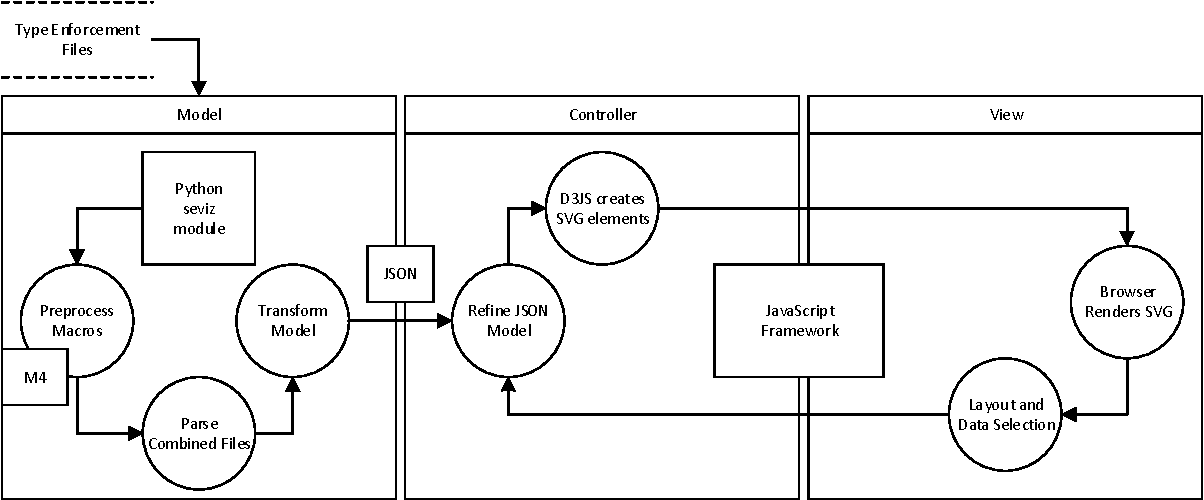
\includegraphics[max width={\textwidth}]{overview.pdf}
\caption{SEUrchin Design Overview}
\label{fig:seurchinoverview}
\end{figure*}

%%%%%%%%%%%%%%%%%%%%%%%%%%%%%%%%%%%%%%%%%%%%%%%%%%%%%%%%%%%%
\subsection{Data Model}\label{sec:datamodel}
The density of the C-libraries, and lack of information originally drove us to writing our own parser, which went through several rounds of development. However, when we found the SELinuxProject's modules \cite{selinuxproject}, we took advantage of a more robust parser that was able to handle all the type enforcement information and store it in the refpolicy model. The Python component of our tool, \texttt{seviz},  handles the parsing and translation of SELinux policy macros and files into JSON data files for our visualization component.

First, we organized the inputs into the build order according to the Android build files of the Android Open Source Project (AOSP)\cite{designandroid}. Next, we utilize \texttt{M4} \cite{m4} to preprocess the attribute and macro files prior to the type enforcements. When working with a reference board policy (e.g. a particular vendor or devices additional policy) it is necessary to interleave these macro files prior to both sets of type enforcements. These steps are complicated, and does not check for compilation errors such as \texttt{allow} rules conflicting with \texttt{neverallow} rules. These could prove beneficial to mark to avoid wasteful compilation, however, for time's sake they are left to future work.

Next, we transform the parsed data model into hierarchical maps that allow multiple layouts to derive their needed information. Types are stored under their classes, which contain children permissions, and finally target types. This model has some minor redundancies in types, and does not allow for constant-time querying like a hash map since the tree's hierarchy must be walked to find types. However, this model is directly accessible to many useful layouts in D3JS, which require tree based data structures. The data set is not massive, so other layouts can quickly derive their own structures with D3JS's powerful data management features. Finally, the data is dumped in JSON format to be immediately accessible to our JavaScript component.

\subsection{Visualization}\label{sec:viz}
The visualization component is a JavaScript framework which leverages the powerful D3JS library\cite{bostock2012d3}. The framework has been designed to be interactive and dynamic. Our initial approach to visualizing these relationships was a traditional network design. However, the nature of access vector (AV) rules in SELinux allows for an explosion of state given complex enough rules\cite{AVCRules}.

We attempted different methods to organize these features including non-expanded macros, a super-graph representing SELinux attribute collections, a network of single types and targets, and a hierarchical edge bundled (HEB) layout\cite{holten2006hierarchical}. SEUrchin's evolution is seen in figure \ref{fig:progress} on page \pageref{fig:progress}.

\begin{figure*}
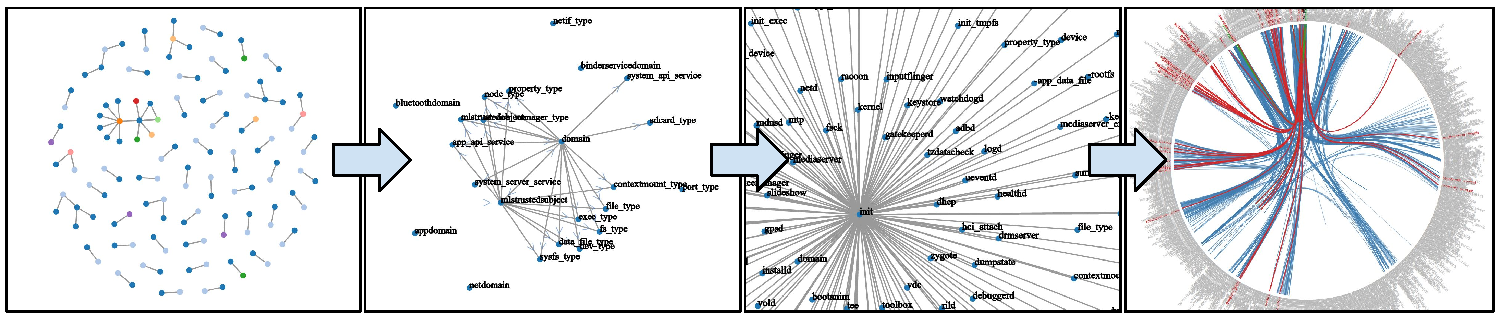
\includegraphics[max width={\textwidth}, frame]{progress-resize.pdf}
\caption{Layout progression. From L to R: non-expanded macros, attribute super-graph, selected node relationships, edge bundled tree cluster}
\label{fig:progress}
\end{figure*}

The network graphs were discarded as too visually cluttered. The HEB provided excellent relationship views, but needed organized. We used classes to group the types instead of attributes because this made more immediate sense in order to focus on process-class types. Thus, we created two layouts for the final product: the interactive tree and HEB.

The tree layout allows the user to search for particular permissions and target sets belonging to a source type. The nodes can be collapsed in order to prevent the entire tree being displayed. An example of the layout is in figure \ref{fig:tree} on page \pageref{fig:tree}. The layout is displaying the \texttt{tcmd} process type object sub-tree of permissions and targets. This example is a relatively small sub-tree in one type for the entire process class. This demonstrates the amount of data that can be stored, but concealed to make it readable in the interactive tree layout. The entire layout can be manipulated with zooming and panning to view different parts or the entirety of the tree. This makes the tree ideal for viewing entire classes of types in one layout. The tree can be re-oriented vertically and horizontally to make reading easier or provide more space for large node sets, respectively.

\begin{figure}
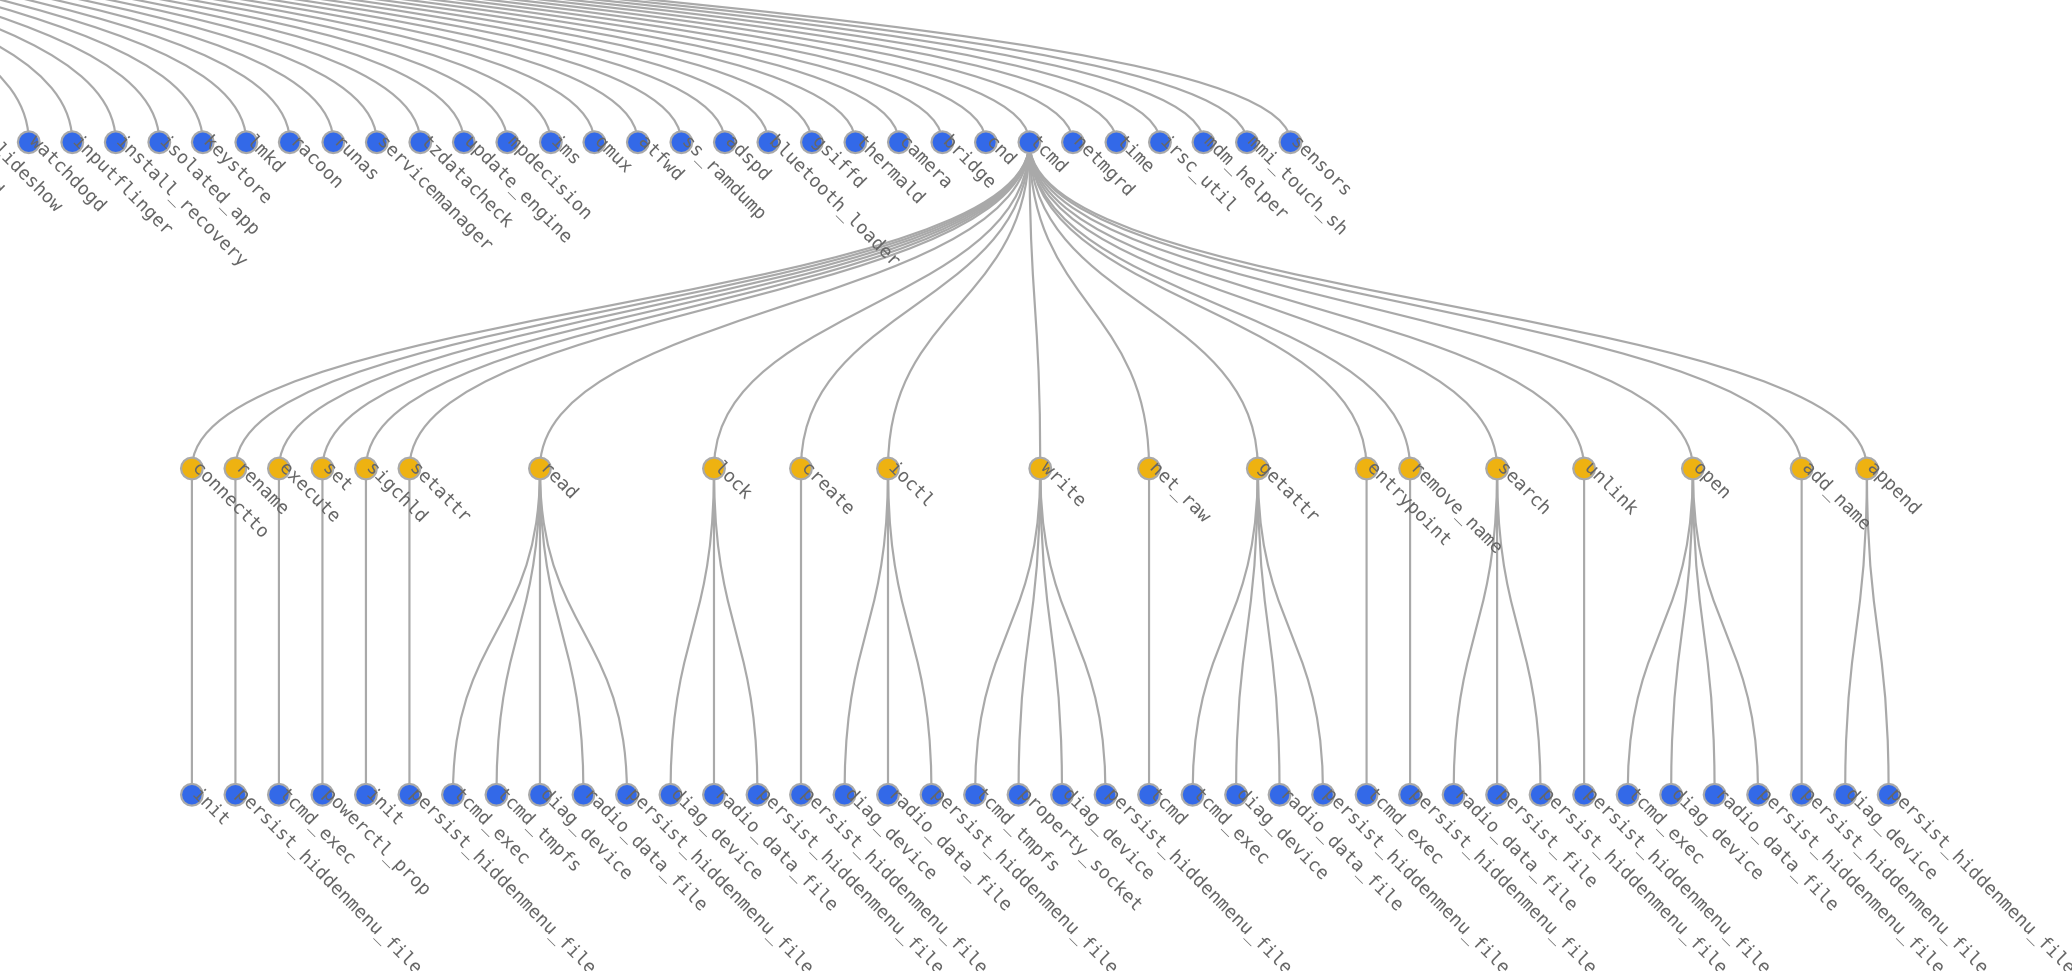
\includegraphics[max width={\columnwidth}, frame]{g5.png}
\caption{Interactive Tree Layout for process \texttt{tcmd}}
\label{fig:tree}
\end{figure}

The HEB is particularly efficient at showing relationships between all permissions and all targets for a particular SELinux type. The visualization in figure \ref{fig:heb} on page \pageref{fig:heb} displays the targets of \texttt{get\_attr} for the \texttt{untrusted\_app} type object. Unlike the tree, you do not need to navigate to each permission and cross-reference the targets (leaf-nodes) mentally. The nodes are centered around a particular type and clustered into targets and permissions which relate to that node. The HEB can highlight all targets of a permission or all permissions of a target by hovering over the node. 

\begin{figure}
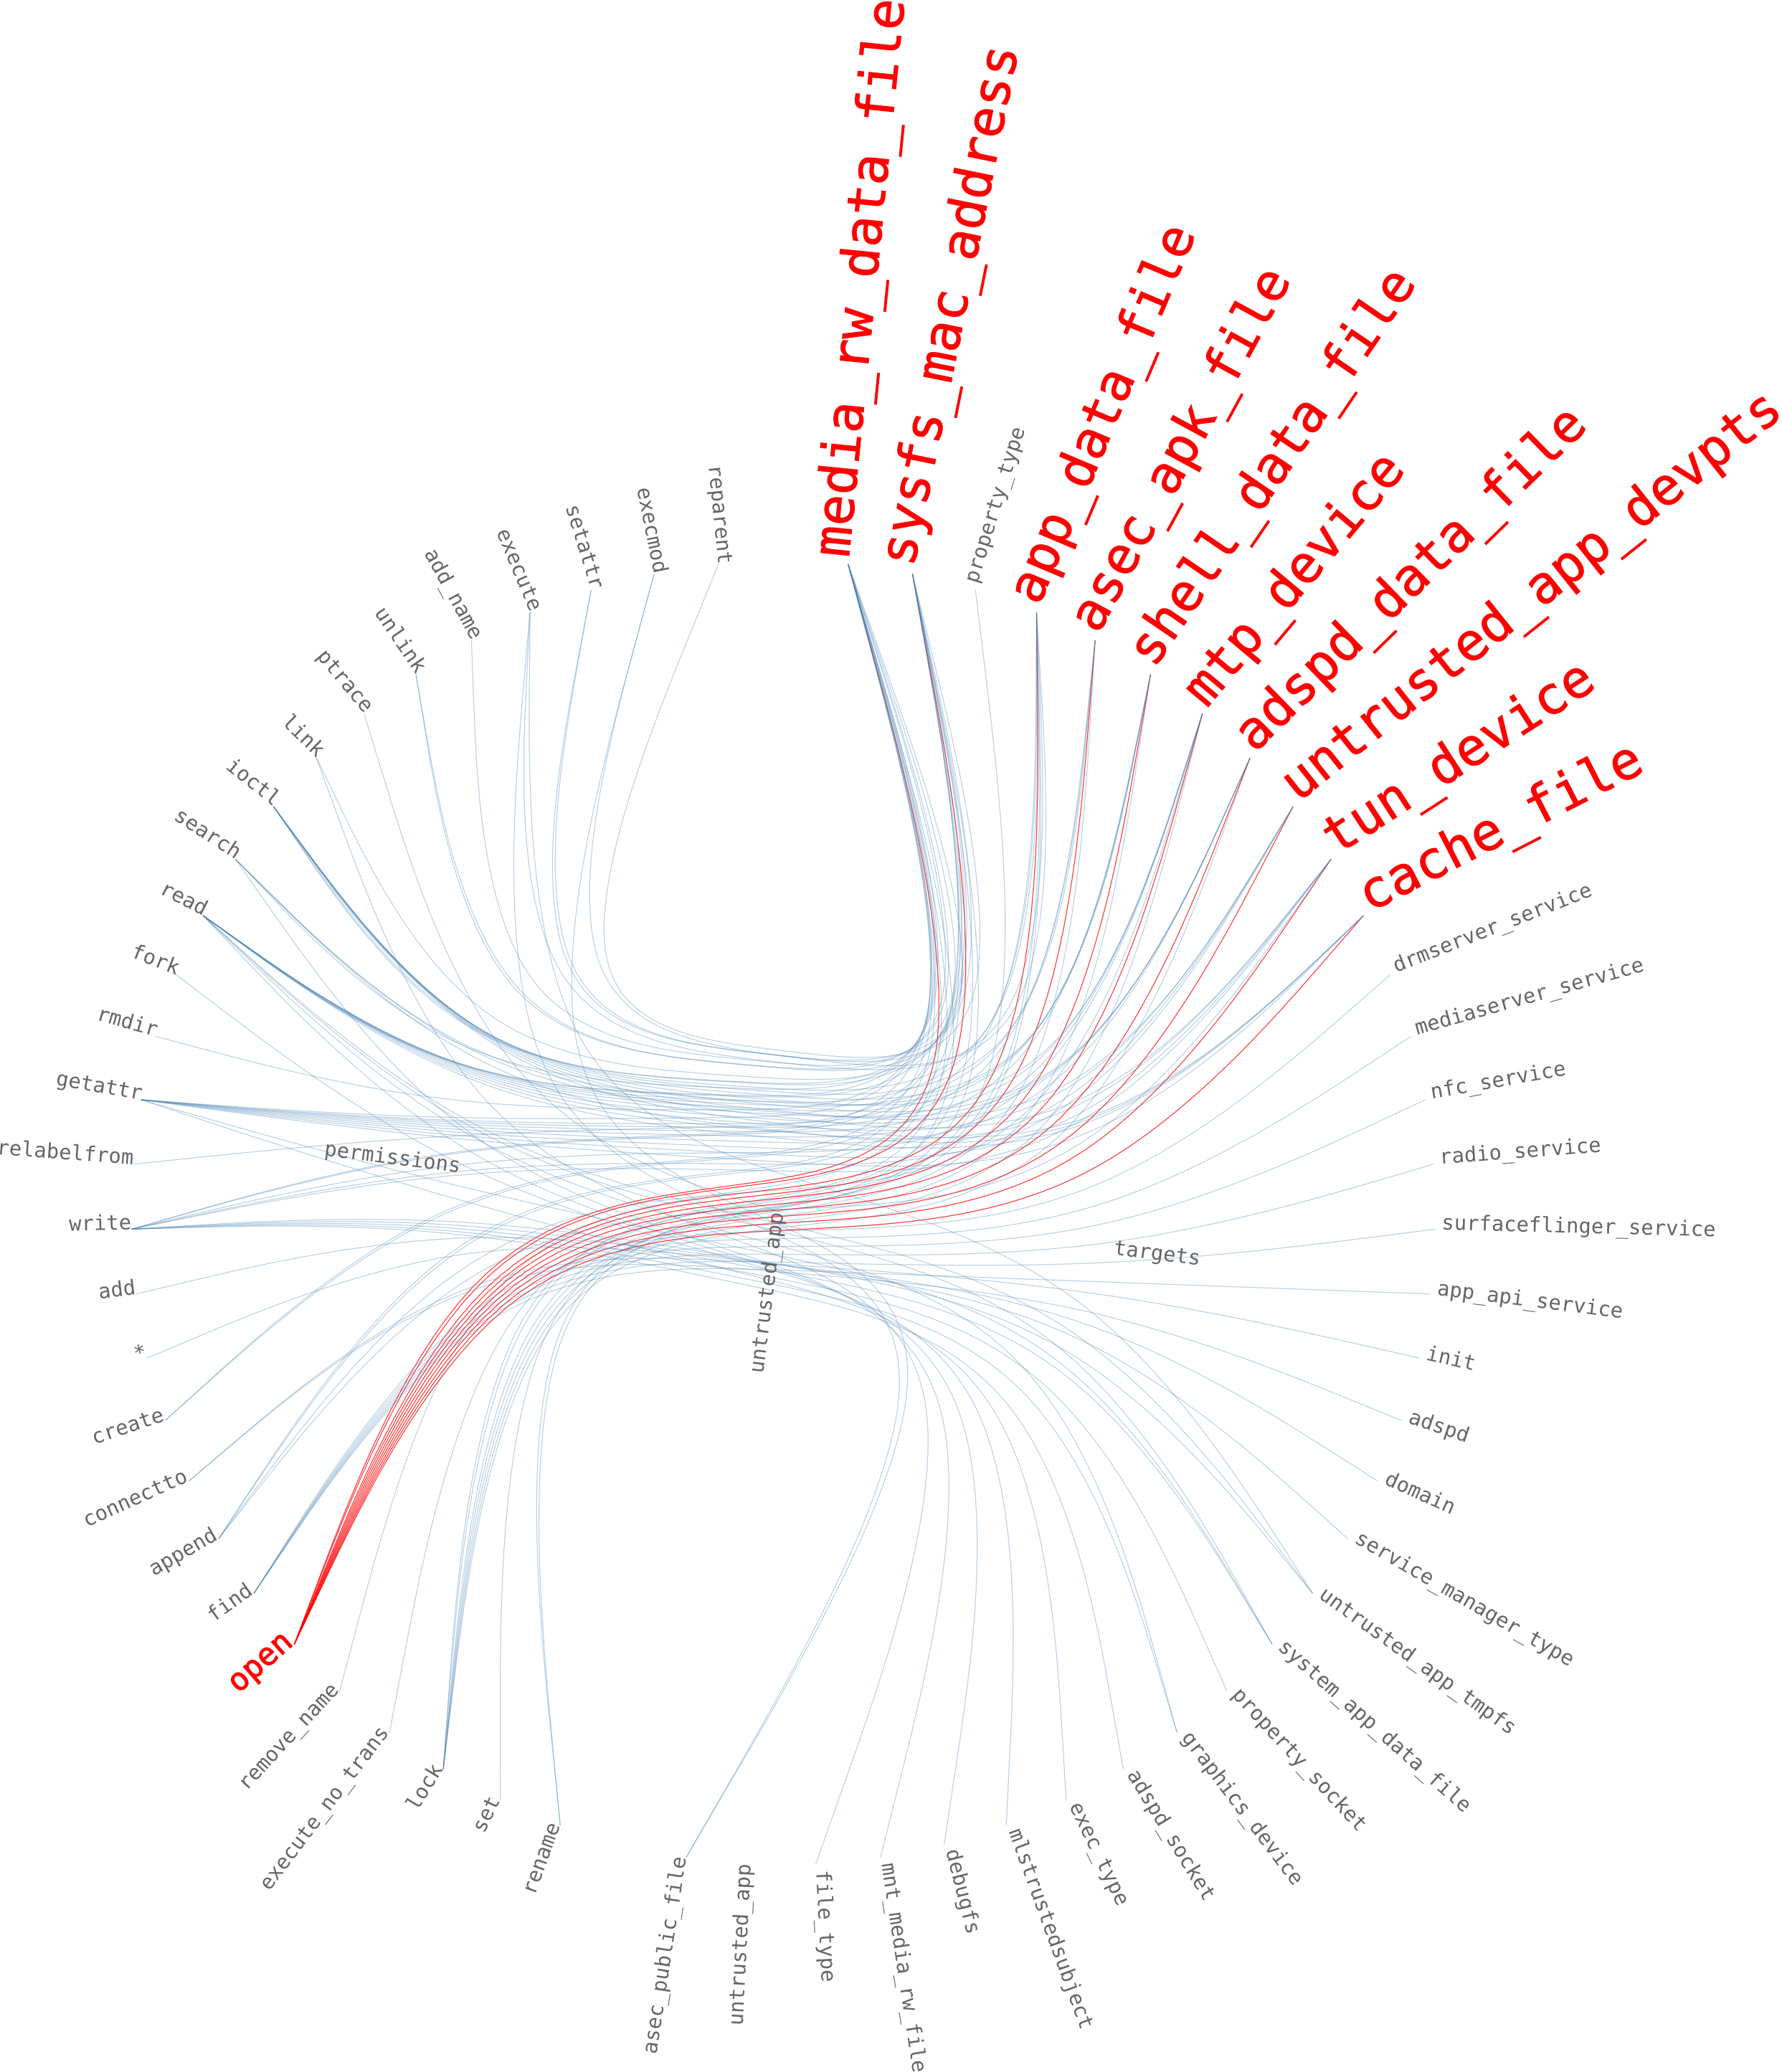
\includegraphics[max width={\columnwidth}, frame]{g4.png}
\caption{Hierarchical Edge Bundle Layout for \texttt{untrusted\_app} type}
\label{fig:heb}
\end{figure}
%%%%%%%%%%%%%%%%%%%%%%%%%%%%%%%%%%%%%%%%%%%%%%%%%%%%%%%%%%%%


%%%%%%%%%%%%%%%%%%%%%%%%%%%%%%%%%%%%%%%%%%%%%%%%%%%%%%%%%%%%
\section{Related Work}\label{sec:related}
%%%%%%%%%%%%%%%%%%%%%%%%%%%%%%%%%%%%%%%%%%%%%%%%%%%%%%%%%%%%
There have been attempts to use visualization as a tool to analyze SELinux policy, or ease its administration \cite{marouf2011segrapher,xu2008visualization}. These tools provide powerful features, but require stand alone programs and installation to use. SELinux's inherent complexity also shows in the visuals produced, which are not very intuitive. Though, a case study on the target audience is really needed to find this out, our tool uses more traditional layouts making it easier for quicker analysis. This project will operate with a stronger set of assumptions because the interest is only in SELinux relationships between types. 

This project also expands on previous work by moving from stand alone complex programs to browser based visualization libraries, such as Raphael\cite{baranovskiy2011raphael}, Protovis\cite{bostock2009protovis}, and D3\cite{bostock2012d3}. Protovis has been discontinued in favor of D3, while Raphael is better equipped to work directly with SVG elements in a browser and has broad legacy browser compatibility. However, we assume that users have up to date systems, and are beginning work with D3, which lacks legacy browser functionality but is well regarded in data visualization.

Very recent work includes projects like SEAL \cite{reshetova2015characterizing}, the SEAndroid Analytics Library. Like our work this library recognizes the need for several new tools to analyze SELinux policy on Android. However, they have not implemented a visualization policy yet, and plan to work with attributes to organize nodes. Our work tried this approach, and along with expert advice decided attributes were not appropriate as described in section \ref{sec:design}.

Previous research on policy query and analysis \cite{archer2003analyzing,marouf2011segrapher,jaeger2003analyzing,zanin2004towards} has created many parsing options. Gokyo\cite{jaeger2003analyzing} is a powerful tool that guarantees a trusted computing base by restricting the set of types to analyze. Additionally, it can detect and suggest resolutions to policy conflicts. However, it verifies the integrity of intentions, but does not reveal unintended relationships that do not result in conflict. Finally, it is not a visualization, and therefore is not as readily accessible by a larger audience. 

Next, SENG is a higher level language for the SELinux policy modules\cite{kuliniewicz2006seng}. While it promises to ease the analysis and management of SELinux by abstracting away complexities, SENG is still a complicated computer language, which does not provide the realizations of visualization tools. Finally, it does not have a decompiler to work backwards from compiled SELinux into SENG, which may be necessary.

Lastly, SELAC \cite{zanin2004towards} is also concerned with the complex relationships that emerge in SELinux, but it is only a proposed model for formal analysis. The authors claim to have built a tool that uses SELAC, and have plans to expand the functionality. However, there has been no update on the research, and the current state does not handle multi-level security (MLS). Our work will lack formal verification, but benefits from the work on SELAC to define relationships from policy types and permissions.
%%%%%%%%%%%%%%%%%%%%%%%%%%%%%%%%%%%%%%%%%%%%%%%%%%%%%%%%%%%%

%%%%%%%%%%%%%%%%%%%%%%%%%%%%%%%%%%%%%%%%%%%%%%%%%%%%%%%%%%%%
\section{Future work}\label{sec:future}
%%%%%%%%%%%%%%%%%%%%%%%%%%%%%%%%%%%%%%%%%%%%%%%%%%%%%%%%%%%%
SEUrchin was designed to be expanded, and has room for improvement. We did not plan for a true user study, which is the real test for all software products. The time-frame of the project and learning curve of our chosen visualization library left some work to be done in the way of features as well. Lastly, there is generally always something to be improved in any program, and SEUrchin may benefit from refactoring our data model.

First and foremost, the tool should be put through a user study. This will inform the directions the tool should take, and provide valuable insight into how it will be used. User studies also assist in finding bugs, and quality control. Because of the complex nature of SELinux, expert users will have very precise notions of what makes the tool useful.

Next, there are some features left to implement. SEUrchin works from source files to quickly analyze policy files without compilation. An obvious way to benefit from this is to image the differences between type enforcement policies before and after a user changes the policy. However, creating differences in the model dictionaries was not done within the time-frame of our work. Also, the tool did not take into account the possibility of catching compilation errors. Our project lead, Jeff Vander Stoep, quickly found these discrepancies testing the latest versions of SEUrchin.

Finally, the data model contains redundancies and may be made more efficient. While most visualizations are CPU limited, this may allow more complicated visualizations by not bogging down the browser window. A better data model can also be designed with stronger querying language, and enable new layouts and user input options. Performance gains would benefit user experience in the form of a more responsive interface.

%%%%%%%%%%%%%%%%%%%%%%%%%%%%%%%%%%%%%%%%%%%%%%%%%%%%%%%%%%%%

%%%%%%%%%%%%%%%%%%%%%%%%%%%%%%%%%%%%%%%%%%%%%%%%%%%%%%%%%%%%
\section{Availability}\label{sec:available}
%%%%%%%%%%%%%%%%%%%%%%%%%%%%%%%%%%%%%%%%%%%%%%%%%%%%%%%%%%%%
SEUrchin is an open source project. It is available with instructions and a demo video on \href{https://github.com/mmaps/selinux/tree/master/policycoreutils/seviz}{our GitHub repository}\cite{SEUrchin}.
%%%%%%%%%%%%%%%%%%%%%%%%%%%%%%%%%%%%%%%%%%%%%%%%%%%%%%%%%%%%
% An example of a floating figure using the graphicx package.
% Note that \label must occur AFTER (or within) \caption.
% For figures, \caption should occur after the \includegraphics.
% Note that IEEEtran v1.7 and later has special internal code that
% is designed to preserve the operation of \label within \caption
% even when the captionsoff option is in effect. However, because
% of issues like this, it may be the safest practice to put all your
% \label just after \caption rather than within \caption{}.
%
% Reminder: the "draftcls" or "draftclsnofoot", not "draft", class
% option should be used if it is desired that the figures are to be
% displayed while in draft mode.
%
%\begin{figure}[!t]
%\centering
%\includegraphics[width=2.5in]{myfigure}
% where an .eps filename suffix will be assumed under latex, 
% and a .pdf suffix will be assumed for pdflatex; or what has been declared
% via \DeclareGraphicsExtensions.
%\caption{Simulation results for the network.}
%\label{fig_sim}
%\end{figure}

% Note that the IEEE typically puts floats only at the top, even when this
% results in a large percentage of a column being occupied by floats.


% An example of a double column floating figure using two subfigures.
% (The subfig.sty package must be loaded for this to work.)
% The subfigure \label commands are set within each subfloat command,
% and the \label for the overall figure must come after \caption.
% \hfil is used as a separator to get equal spacing.
% Watch out that the combined width of all the subfigures on a 
% line do not exceed the text width or a line break will occur.
%
%\begin{figure*}[!t]
%\centering
%\subfloat[Case I]{\includegraphics[width=2.5in]{box}%
%\label{fig_first_case}}
%\hfil
%\subfloat[Case II]{\includegraphics[width=2.5in]{box}%
%\label{fig_second_case}}
%\caption{Simulation results for the network.}
%\label{fig_sim}
%\end{figure*}
%
% Note that often IEEE papers with subfigures do not employ subfigure
% captions (using the optional argument to \subfloat[]), but instead will
% reference/describe all of them (a), (b), etc., within the main caption.
% Be aware that for subfig.sty to generate the (a), (b), etc., subfigure
% labels, the optional argument to \subfloat must be present. If a
% subcaption is not desired, just leave its contents blank,
% e.g., \subfloat[].


% An example of a floating table. Note that, for IEEE style tables, the
% \caption command should come BEFORE the table and, given that table
% captions serve much like titles, are usually capitalized except for words
% such as a, an, and, as, at, but, by, for, in, nor, of, on, or, the, to
% and up, which are usually not capitalized unless they are the first or
% last word of the caption. Table text will default to \footnotesize as
% the IEEE normally uses this smaller font for tables.
% The \label must come after \caption as always.
%
%\begin{table}[!t]
%% increase table row spacing, adjust to taste
%\renewcommand{\arraystretch}{1.3}
% if using array.sty, it might be a good idea to tweak the value of
% \extrarowheight as needed to properly center the text within the cells
%\caption{An Example of a Table}
%\label{table_example}
%\centering
%% Some packages, such as MDW tools, offer better commands for making tables
%% than the plain LaTeX2e tabular which is used here.
%\begin{tabular}{|c||c|}
%\hline
%One & Two\\
%\hline
%Three & Four\\
%\hline
%\end{tabular}
%\end{table}


% Note that the IEEE does not put floats in the very first column
% - or typically anywhere on the first page for that matter. Also,
% in-text middle ("here") positioning is typically not used, but it
% is allowed and encouraged for Computer Society conferences (but
% not Computer Society journals). Most IEEE journals/conferences use
% top floats exclusively. 
% Note that, LaTeX2e, unlike IEEE journals/conferences, places
% footnotes above bottom floats. This can be corrected via the
% \fnbelowfloat command of the stfloats package.



%%%%%%%%%%%%%%%%%%%%%%%%%%%%%%%%%%%%%%%%%%%%%%%%%%%%%%%%%%%%
\section{Conclusion}\label{sec:conclusion}
SEUrchin is an interactive SELinux source policy visualization tool that enables faster policy analysis. SEUrchin is capable of analyzing type enforcement files with preprocessing of macros using \texttt{M4} \cite{m4}. The tool has two current layouts, which provide different results. The tree is useful for examining larger type sets and type classes, while the edge bundled clusters are useful for displaying relationships from permissions to targets and targets to permissions for a particular source type. SEUrchin is hosted publicly, and was designed to be accessible for future work.
%%%%%%%%%%%%%%%%%%%%%%%%%%%%%%%%%%%%%%%%%%%%%%%%%%%%%%%%%%%%





% use section* for acknowledgment
%%%%%%%%%%%%%%%%%%%%%%%%%%%%%%%%%%%%%%%%%%%%%%%%%%%%%%%%%%%%
\section*{Acknowledgment}\label{sec:ack}

The authors would like to thank our technical director for our research, Jeff Vander Stoep for his patience and helpful criticisms, as well as our professor, Patrick Tague and the super awesome teaching assistants of the 14-829/18-638 Mobile Security course at CMU, Nandita Joshi and Brian Ricks for their continued guidance and support. 
%%%%%%%%%%%%%%%%%%%%%%%%%%%%%%%%%%%%%%%%%%%%%%%%%%%%%%%%%%%%




% trigger a \newpage just before the given reference
% number - used to balance the columns on the last page
% adjust value as needed - may need to be readjusted if
% the document is modified later
%\IEEEtriggeratref{8}
% The "triggered" command can be changed if desired:
%\IEEEtriggercmd{\enlargethispage{-5in}}

% references section

% can use a bibliography generated by BibTeX as a .bbl file
% BibTeX documentation can be easily obtained at:
% http://mirror.ctan.org/biblio/bibtex/contrib/doc/
% The IEEEtran BibTeX style support page is at:
% http://www.michaelshell.org/tex/ieeetran/bibtex/
\bibliographystyle{IEEEtran}
% argument is your BibTeX string definitions and bibliography database(s)
\bibliography{IEEEabrv,main.bib}
%
% <OR> manually copy in the resultant .bbl file
% set second argument of \begin to the number of references
% (used to reserve space for the reference number labels box)

%\begin{thebibliography}{1}

%\end{thebibliography}




% that's all folks
\end{document}